\documentclass[useAMS,usenatbib]{mn2e}
\usepackage{footnote}
\usepackage{graphicx}
\usepackage{amsmath}
\usepackage{natbib}
\usepackage{array}
\usepackage{color}
\usepackage{url}
\voffset=-0.5in

\definecolor{nc}{rgb}{0,0,0}
\def\changed    {\color{nc} }

\def\starpy {\textsc{starpy}}

\begin{document}
\title[AGN & Star Formation]{Galaxy Zoo: Two modes of black hole growth driven by star formation}
\author[Smethurst et al. 2014]{R. ~J. ~Smethurst,$^{1}$ C. ~J. ~Lintott,$^{1}$ B. ~D. ~Simmons,$^{1}$
\\ $^1$ Oxford Astrophysics, Department of Physics, University of Oxford, Denys Wilkinson Building, Keble Road, Oxford, OX1 3RH, UK 
\\
}

\maketitle

\begin{abstract}
Two modes of black hole growth in early and late type galaxies but no correlation to mechanisms. New Bayesian SFH tool \starpy let's us investigate the SFH as two parameters $[t, \tau]$ and investigate the AGN fraction, duty cycle and average AGN luminosity across this parameter space. We find that rapid quenching mechanisms give rise to high luminosity AGN and slow quenching mechanisms to low luminosity AGN.\footnotemark[1]

\end{abstract}

\footnotetext[1]{This investigation has been made possible by the participation of more than 250,000 users in the Galaxy Zoo project. Their contributions are individually acknowledged at \url{http://authors.galaxyzoo.org}}

\section{Introduction}

There is clearly a relationship between central black hole and evolution of galaxy. Magorrian relation shows this as do simulations and observations of feedback. 

This effect seems to be strongest during AGN phase of black hole growth. 

Previous studies shown that two different modes of black hole growth in late types and early types. 

Largest fraction of AGN found in green valley suggesting some link to the process of quenching star formation in order for a galaxy to progress from the blue cloud to the red sequence. 

Here we try to link the star formation history of galaxies to the presence of AGN with the use of novel new Bayesian code \starpy which given NUV and optical colours and using SSP models can effectively describe the SFH of a galaxy with two parameters. 


\section{Data}

\subsection{Galaxy Zoo 2}\label{galzoo}

Galaxy Zoo is awesome. Especially GZ2 which provides us with a huge probabilistic data set with reliable morphological classifications of a huge set of galaxies. 

\begin{figure*}
\centering{
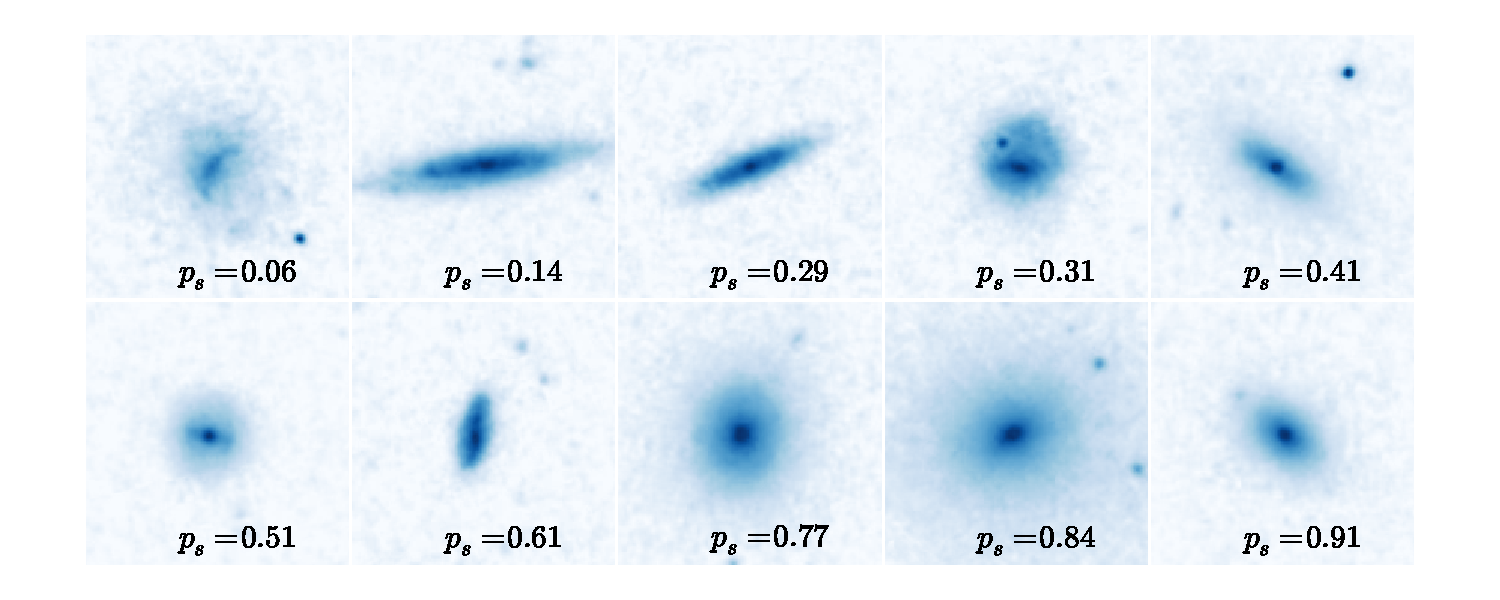
\includegraphics[width=\textwidth]{mosaic_agn_smooth_fraction.pdf}}
\caption{{\newchange Randomly selected SDSS \emph{gri} composite images showing the continuous probabilistic nature of the Galaxy Zoo sample from a redshift range $0.040 < z < 0.045$. The debiased smooth vote fraction (see \citealt{GZ2}) for each galaxy is shown. The scale for each image is $0.099~\rm{arcsec/pixel}$.}}
\label{mosaic}
\end{figure*}


\subsection{\sc{STARPY}}

\starpy is awesome. It gives Bayesian derived quenched SFHs of galaxies described by two parameters. We used it and described it fully in \cite{Sme2015}. 

\subsection{AGN Selection}

\cite{Sch2010} made a sample of AGN from GZ - it is publicly available on the web. These galaxies have been run through \starpy to get the best description of their quenched star formation histories. 

\section{Results}

Here are all the ridiculous amounts of plots I made condensed down into 1 or 2 easy to understand plots that gets the point across. 

\section{Discussion}

Rapid quench results in high luminosity AGN. 

Slow quench results in low luminosity AGN. 

Majority of disc galaxies with AGN found at slow quenching timescales but with low luminosity AGN. 

Small fraction of AGN are in smooth galaxies found at rapid quenching timescales with high luminosity AGN. 

Two modes of black hole growth clearly highlighted. 

\section{Conclusion}

AGN and SFH linked. Rapid == high luminosity but there's not a lot of those. Slow == low luminosity and there's loads of those. 

\section*{Acknowledgements}

RS acknowledges funding from the Science and Technology Facilities Council Grant Code ST/K502236/1. BDS gratefully acknowledges support from the Oxford Martin School, Worcester College and Balliol College, Oxford. KS gratefully acknowledges support from Swiss National Science Foundation Grant PP00P2\_138979/1.

The development of Galaxy Zoo was supported in part by the Alfred P. Sloan Foundation. Galaxy Zoo was supported by The Leverhulme Trust. 

Based on observations made with the NASA Galaxy Evolution Explorer.  GALEX is operated for NASA by the California Institute of Technology under NASA contract NAS5-98034

Funding for the SDSS and SDSS-II has been provided by the Alfred P. Sloan Foundation, the Participating Institutions, the National Science Foundation, the U.S. Department of Energy, the National Aeronautics and Space Administration, the Japanese Monbukagakusho, the Max Planck Society, and the Higher Education Funding Council for England. The SDSS Web Site is \url{http://www.sdss.org/}.
The SDSS is managed by the Astrophysical Research Consortium for the Participating Institutions. The Participating Institutions are the American Museum of Natural History, Astrophysical Institute Potsdam, University of Basel, University of Cambridge, Case Western Reserve University, University of Chicago, Drexel University, Fermilab, the Institute for Advanced Study, the Japan Participation Group, Johns Hopkins University, the Joint Institute for Nuclear Astrophysics, the Kavli Institute for Particle Astrophysics and Cosmology, the Korean Scientist Group, the Chinese Academy of Sciences (LAMOST), Los Alamos National Laboratory, the Max-Planck-Institute for Astronomy (MPIA), the Max-Planck-Institute for Astrophysics (MPA), New Mexico State University, Ohio State University, University of Pittsburgh, University of Portsmouth, Princeton University, the United States Naval Observatory, and the University of Washington.

This publication made extensive use of the Tool for Operations on Catalogues And Tables (TOPCAT; ~\citealt{Taylor05}) which can be found at \url{http://www.star.bris.ac.uk/~mbt/topcat/}. Ages were calculated from the observed redshifts using the \emph{cosmolopy} package provided in the Python module \emph{astroPy}\footnote{\url{http://www.astropy.org/}}; \citealt{Rob13}). This research has also made use of NASA's ADS service and Cornell's ArXiv. 

\begin{thebibliography}{}

\bibitem[\protect\citeauthoryear{Lintott et al.}{2008}]{Lintott09} Lintott, C. J. et al., 2008, MNRAS, 389, 1179

\bibitem[\protect\citeauthoryear{Lintott et al.}{2011}]{Lintott11} Lintott, C. J. et al., 2011, MNRAS, 410, 166

\bibitem[\protect\citeauthoryear{Robitaille et al.}{2013}]{Rob13} Robitaille, T. P. et al., 2013, A\&A, 558, A33

\bibitem[\protect\citeauthoryear{Schawinski et al.}{2010}]{Sch2010} Schawinski, K. et al., 2010, MNRAS, 711, 284

\bibitem[\protect\citeauthoryear{Smethurst et al.}{2015}]{Sme2015} Smethurst, R. J. et al., 2015, arXiv: 1501.05955

\bibitem[\protect\citeauthoryear{Taylor}{2005}]{Taylor05} Taylor, M. B., 2005, ASP Conference Series, 347

\bibitem[\protect\citeauthoryear{Willett et al.}{2013}]{GZ2} Willett, K. et al., 2013, MNRAS, 435, 2835

\end{thebibliography}{}

\appendix

\end{document}
